\documentclass[11pt, oneside]{article}   	% use "amsart" instead of "article" for AMSLaTeX format
%\usepackage{geometry}                		% See geometry.pdf to learn the layout options. There are lots.
%\geometry{letterpaper}                   		% ... or a4paper or a5paper or ... 
%\geometry{landscape}                		% Activate for rotated page geometry
%\usepackage[parfill]{parskip}    		% Activate to begin paragraphs with an empty line rather than an indent

\usepackage{geometry}
 \geometry{
 a4paper,
 total={170mm,257mm},
 left=20mm,
 top=25mm,
 bottom=25mm
 }

\usepackage{graphicx}				% Use pdf, png, jpg, or eps§ with pdflatex; use eps in DVI mode
								% TeX will automatically convert eps --> pdf in pdflatex		
\usepackage{amssymb}
\usepackage{amsmath}
\usepackage{fancyhdr}
\usepackage[utf8]{inputenc}
\usepackage[english]{babel}
\usepackage{enumerate}
\usepackage{arcs}
\usepackage{cancel}
\usepackage{xfrac}
\usepackage{amsthm}
\usepackage{gensymb}
\usepackage{xspace}

\usepackage{epigraph}
\usepackage{csquotes}
\usepackage{soul}
\usepackage{subcaption}
%\usepackage{ctex}

%SetFonts

%SetFonts

\usepackage[inline]{asymptote}


\pagestyle{fancy}
\fancyhf{}
%\rhead{Teacher David}
\lhead{\leftmark}
%\lfoot{Copyright \copyright 2021-2022 by Teacher David. All rights reserved.}

\title{USBL Notes}
\author{Teacher David}
\date{January 12, 2023}							% Activate to display a given date or no date

\newcommand{\latex}{\LaTeX\xspace}


\begin{document}
\maketitle

\section{USBL Positioning}
\begin{quotation}
``\emph{The USBL transceiver measures the time from transmission of its acoustic signal until an acoustic reply from the transponder is detected, and converts it to distance to the transponder. Containing several transducers separated by a short distance (the ultra-short baseline antenna), the transceiver calculates the angle to the transponder}.'' -- From the S2C Reference Manual.
\end{quotation}

\subsection{Positioning Strings}

\textbf{USBLLONG}

\textbf{USBLANGLES}


\textbf{USBLPHYP}

\textbf{USBLPHYD}


\newpage
\section{Inertial Measurement Unit: ICM20948}

\begin{figure}[ht]
\centering
\begin{subfigure}[b]{0.45\textwidth}
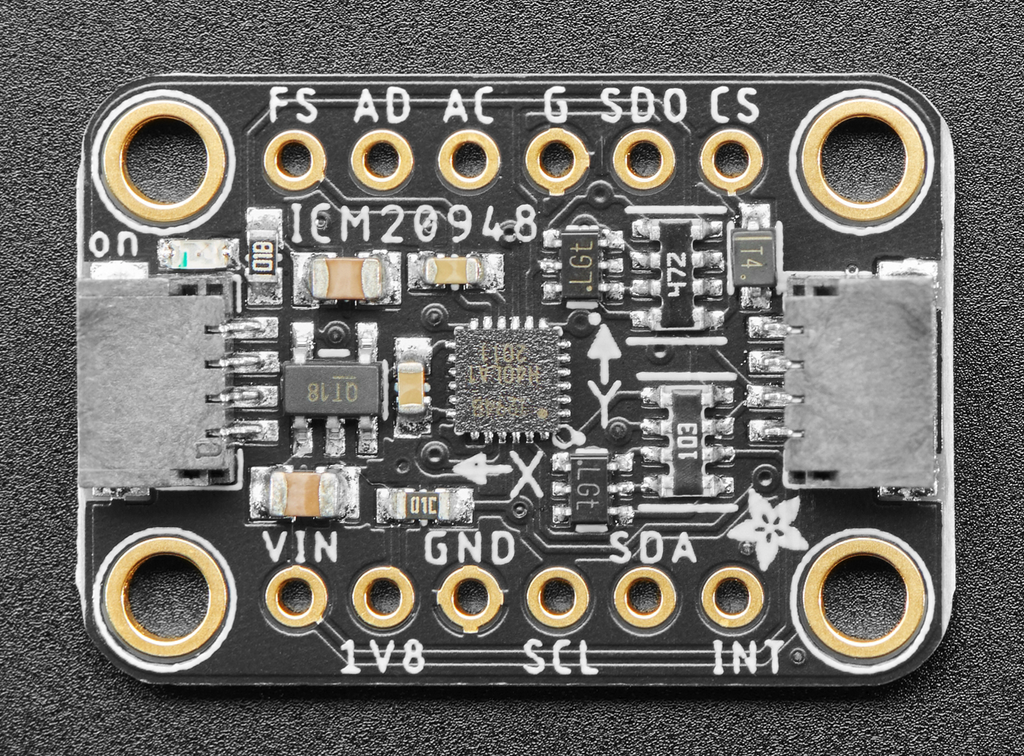
\includegraphics[width=\textwidth]{imgs/icm20948-front.png}
\caption{ICM20948 Front}
\end{subfigure}
\begin{subfigure}[b]{0.45\textwidth}
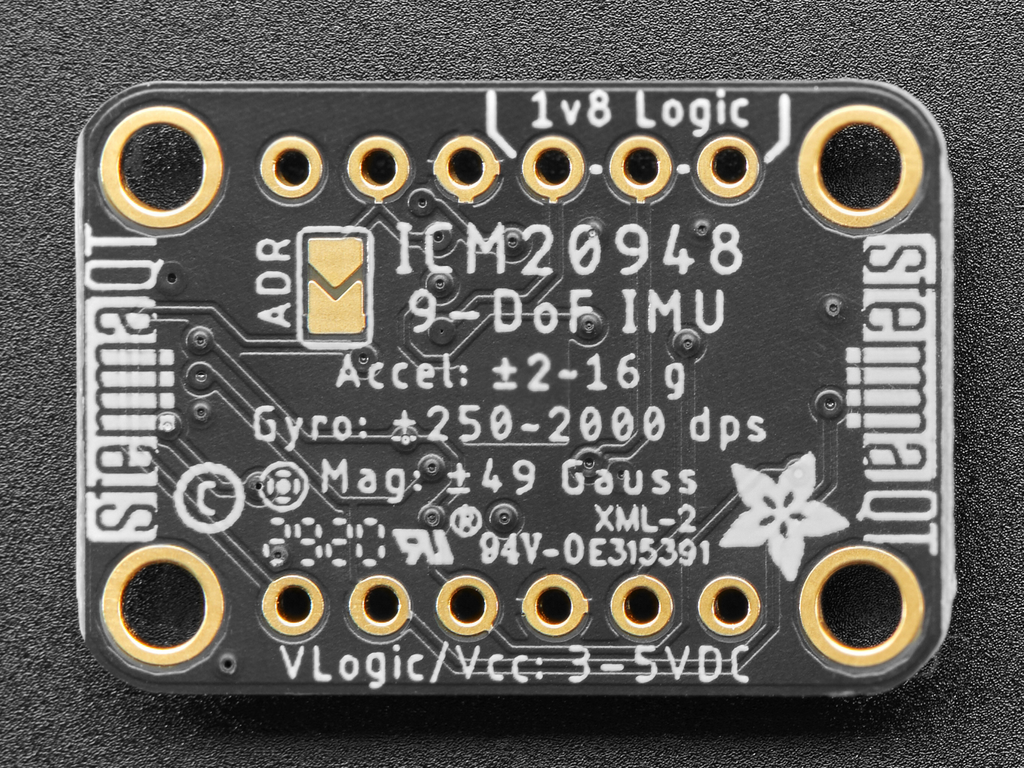
\includegraphics[width=\textwidth]{imgs/icm20948-back.png}
\caption{ICM20948 Back}
\end{subfigure}
\end{figure}

\begin{center}
\begin{asy}
/* 
ICM20948 board: 15.7mm x 17.7mm x 4.6mm (1'' x 0.7'' x 0.2'');
24-pin QFN: 3mm x 3mm x 1mm
*/
import math;
unitsize(16pt);
int h = 7;
int w = 10;
real r = 0.7;
draw(box((0,0),(w,h)));

pair [] p1 = {(1,1), (w-1,1), (1,h-1), (w-1,h-1)};
for (int i=0; i<p1.length; ++i) {
    draw(circle(p1[i], r));
    draw(circle(p1[i], r-0.1));
}

void plotoutpins(pair a, pair b, string [] a1, string [] b1, real gapx, real gapt, real r) {
    for (int i=0; i<a1.length; ++i) {
        pair x = a+i*(gapx, 0);
        draw(circle(x, r/2));
        label("\tiny "+a1[i], x-(0,gapt), S);
        pair y = b+i*(gapx, 0);
        draw(circle(y, r/2));
        label("\tiny "+b1[i], y+(0,gapt), N);
    }
}

string [] a1 = {"VIN", "1V8", "GND", "SCL", "SDA", "INT"};
string [] b1 = {"FS", "AD", "AC", "G", "SD0", "CS"};

plotoutpins((2.5,1), (2.5,h-1), a1, b1, 1, 0.3, r);

draw(box((0.1, 2.15), (1+r, 4.85)));
draw(box((w-0.1, 2.15), (w-1-r, 4.85)));

for (int i=0; i<4; ++i) {
    filldraw(box((0.9+r,2.8+i*0.4),(1.3+r,3+i*0.4)), gray);
    draw((0.8+r,2.9+i*0.4)--(1+r,2.9+i*0.4));
    filldraw(box((w-0.9-r,2.8+i*0.4),(w-1.3-r,3+i*0.4)), gray);
    draw((w-0.8-r,2.9+i*0.4)--(w-1-r,2.9+i*0.4));    
}

void plotaxis(pair o) {
    dot(o);
    pair x = o - (1.2,0);
    pair y = o + (0,1.2);
    draw(o -- x, arrow=Arrow(TeXHead), blue);
    draw(o -- y, arrow=Arrow(TeXHead), blue);
    label("\small $x$", (o+x)/2, S);
    label("\small $y$", (o+y)/2, E);
}

plotaxis((6.2, 2.3));

void drawcenterunit(pair o) {
  real w = 1.16;
  real gap = 0.16;
  pair a = o - 0.5*(w,w), b = o+0.5*(w,w);
  draw(box(a, b));
  
  real t = (w - 5*gap)/2;
  real k = 0.1;
  for (int i=0; i<6; ++i) {
    draw((a.x+t+i*gap, b.y)--(a.x+t+i*gap,b.y+k));
    draw((a.x+t+i*gap, a.y)--(a.x+t+i*gap,a.y-k)); 
    draw((a.x, a.y+t+i*gap)--(a.x-k,a.y+t+i*gap)); 
    draw((b.x, a.y+t+i*gap)--(b.x+k,a.y+t+i*gap)); 
  }
}

drawcenterunit((5,3.5));
label("\small ICM20948", (1+r, 4.85), E);
\end{asy}
\end{center}

\subsection{Pinouts}
\subsubsection{Power Pins}
\begin{enumerate}
\item VIN: This is the power pin. Since the sensor chip uses 3 VDC, we have included a voltage regulator on board that will take 3-5VDC and safely convert it down. To power the board, give it the same power as the logic level of your microcontroller (e.g. for a 5V microcontroller like Arduino, use 5V).
\item 1V8: This is the 1.8V output from the voltage regulator, you can grab up to 100mA from this if you like.
\item GND: The common ground for power and logic.
\end{enumerate}

\subsubsection{I2C Logic Pins}
\begin{enumerate}
\item SCL: I2C clock pin, connect to your microcontroller I2C clock line. This pin is level shifted so you can use 3-5V logic, and there's a 10K pullup on this pin.
\item SDA: I2C data pin, connect to your microcontroller I2C data line. This pin is level shifted so you can use 3-5V logic, and there's a 10K pullup on this pin.
\item STEMMA QT: These connectors allow you to connectors to dev boards with STEMMA QT connectors or to other things with various associated accessories.
\item SDO/ADR Jumper: I2C Address pin. Pulling this pin high or bridging the solder jumper on the back will change the I2C address from 0x69 to 0x68.
\end{enumerate}

\subsubsection{SPI Logic Pins}
\begin{enumerate}
\item SCL: This is also the SPI Clock pin / SCK, it's an input to the chip.
\item SDA: This is also the Serial Data In / Microcontroller Out Sensor In / MOSI pin, for data sent from your processor to the ICM20948.
\item SDO: This is the Serial Data Out / Microcontroller In Sensor Out / MISO pin, for data sent from the ICM20948 to your processor. 
\item CS: This is the Chip Select pin, drop it low to start an SPI transaction. It's an input to the chip.
\end{enumerate}

\subsubsection{Other Pins}
\begin{enumerate}
\item INT: This is the primary interrupt pin. You can setup the ICM20948 to pull this low or high when certain conditions are met such as new measurement data being available. Consult the datasheet for usage
\item AC: Auxillary I2C bus clock. Advanced users can consult the datasheet to learn how to use this pin to communicate with sensors on the ICM20948's auxiliary bus. 1.8V Logic Only!
\item AD: Auxiliary I2C bus data. Advanced users can consult the datasheet to learn how to use this pin to communicate with sensors on the ICM20948's auxiliary bus. 1.8V Logic Only!
\item FS:  External frame sync. Advanced users can consult the datasheet to learn how to use this pin to synchronize measurements with additional sensors. 1.8V Logic Only!
\end{enumerate}

\subsubsection{Note}
If you want to connect multiple ICM20948s to one microcontroller, have them share the SCL, SDA, and DO pins. Then assign each one a unique CS pin.

\end{document} 